\documentclass[10pt,letterpaper]{article}
\usepackage[utf8]{inputenc}
\usepackage[T1]{fontenc}
\usepackage{mathptmx}
\usepackage[scaled=0.92]{helvet}
\usepackage{courier}
\usepackage{graphicx, geometry, amsmath, amssymb, hyperref, url, booktabs, xcolor, array, caption, microtype, xurl}
\geometry{margin=0.85in}
\hypersetup{colorlinks=true, linkcolor=black, citecolor=black, urlcolor=black}
\captionsetup{font=small}
\setlength{\parskip}{3pt}
\setlength{\parindent}{0pt}
\newcolumntype{L}[1]{>{\raggedright\arraybackslash\hspace{0pt}}p{#1}}
\title{Steering a 3B Code Model Selects One Known Algorithm Rather Than Diversifying\\[3pt]\large Executive summary of the run}
\date{16 October 2026}
\author{}
\begin{document}
\maketitle
\vspace{-2.5em}

\section*{1. Headline}

\textbf{Away-from-mode steering selects one predicted algorithm family rather than flattening the distribution.} In a pre-registered test on Qwen2.5-3B-Instruct, the test's rules, strengths and predicted gainers were frozen by hash before the main runs. A difference-in-means direction pointing away from the model's default algorithm met the frozen SELECT rule on both tasks, on the main draw and on a fresh-seed re-draw. On sorting in the re-draw (seeds 1000 to 1149, strength s2, $\alpha = 0.473$, n = 150), bubble sort fell from 62\% of programs to 0\% and quicksort, the predicted gainer, rose to 68\%. Entropy over algorithm families was 1.022 bits against a mean of 1.749 bits over five matched-norm random directions. The difference is $-0.727$ bits, 95\% CI $[-0.954, -0.451]$ (Miller-Madow entropy, hierarchical bootstrap over draws and samples, 10,000 resamples). The pass rate was 0.913 against 0.984 for the random-draw mean. \emph{Source:} artifact gen\_art\_experiment\_6, round 2 (report Table~73). We checked these values against the artifact's \texttt{results/selector\_tables.json} and they match.

\emph{Evidence grade.} The frozen rule's verdict is SELECT on both tasks and both draws. The round-2 record grades this strand \emph{lead}, not confirmed: review score 5, non-blocking. \textbf{Conflict:} the paper states the result as a passed pre-registered test, while the round record keeps it at ``lead'' because of three caveats. The direction built for the other task also moves path search to A$^*$ (40 of 150). Individual random draws also move sorting a lot (random mode share 0.19 to 0.69). And the path-search operating point missed its frozen pass-rate bar (pass 0.17, against 0.31 at baseline).

\emph{Scope.} One 3B model, the HF engine, one bare prompt wording per task, two tasks. The SELECT rule accepted the top gainer of either of two frozen rankings; the projection ranking was right on both tasks and the nearest-neighbour ranking was wrong on both. Selection reaches only ideas the model already writes.

\section*{2. Goal}

The run asked how an instruction-tuned open-weight model chooses the solution idea for an open coding task (for example, which path-search or sorting algorithm it writes), and whether that choice can be pushed toward ideas the model does not usually produce. The knobs were temperature and top-k, random seed strings, prompt instructions (bans, mentions, novelty requests) and internal edits (activation steering, concept erasure). Every program was labelled by an audited classifier and checked by execution, so that a change of idea could be told apart from a change of wording, and a correct new program from a broken one.

\section*{3. What was tried}

\textbf{Round 1.} A pre-registered three-arm screen on Qwen2.5-3B-Instruct (temperature, bans, internal knobs), with survival rules frozen before data existed. Only the influence arm, gen\_art\_experiment\_3, was analysed at the time: 19,250 generations comparing steering and erasure with temperature, novelty prompts, a top-3 ban and generate-then-select, on two path tasks whose prompts carried a fixed output contract. No internal knob survived. The reviewer blocked the round (score 4) for two reasons: the other two arms had left thousands of unanalysed generations on disk, and the output contract had narrowed each task to a two-idea menu.

\textbf{Round 2.} All core tests moved to the user's bare prompt. gen\_art\_experiment\_4 labelled and executed 13,968 programs with one audited classifier, wrote up the round-1 ban arm, and tested a frozen temperature law and a frozen seed-shock predictor on fresh draws. gen\_art\_experiment\_5 treated bans as displacements of the prompt-final residual stream: it froze seven substitution predictors and scored them on 5,930 never-generated confirmation programs (including a new k-th-smallest task), then ran transplant and attention-knockout tests. gen\_art\_experiment\_6 re-analysed the round-1 random-control claim, ran the pre-registered select-or-flatten test, and repeated the ban and temperature tests on gemma-2-2b-it. The reviewer scored the round 5, non-blocking.

\section*{4. Key results}

\begin{center}
\footnotesize
\setlength{\tabcolsep}{3pt}
\begin{tabular}{@{}L{0.30\linewidth}L{0.37\linewidth}L{0.13\linewidth}L{0.15\linewidth}@{}}
\toprule
\textbf{Finding} & \textbf{Numbers} & \textbf{Source} & \textbf{Grade (round record)} \\
\midrule
Steering away from the default selects the predicted idea (headline) & Sorting re-draw: entropy $-0.727$ $[-0.954, -0.451]$ vs random mean; quicksort 65\%/68\%. Path search: A$^*$ 57\%/63\%, pass 0.17 vs 0.337 (random mean) & gen\_art\_exp.\_6, round 2 & frozen rule met; strand ``lead'' \\
The bare-prompt default is the mode of a small menu & Path search: BFS 179, DFS 44, A$^*$ 39, Dijkstra 22 of 300; weighted task: Dijkstra 300 of 300 & gen\_art\_exp.\_4, round 2 & descriptive \\
Temperature adds ideas slowly and breaks code & Path search, T 0.3 to 1.0: entropy 1.698 to 1.962 bits, pass 0.49 to 0.19; frozen temperature law met on no task & gen\_art\_exp.\_4, round 2 & law failed (pre-registered) \\
Seed strings narrow the ideas & Entropy change at T = 0.7: $-0.337$ $[-0.529, -0.132]$ (path), $-0.677$ $[-0.917, -0.467]$ (sorting) & gen\_art\_exp.\_4, round 2 & ``lead''; predictor failed \\
Bans lower ideas they do not name & 8 of 46 cells at Holm p $<$ 0.01, 0 of 45 placebo-vs-placebo; banning greedy best-first: A$^*$ 3\% to 58\% & gen\_art\_exp.\_5, round 2 & passed (pre-registered); ``lead'' \\
Internal displacement barely beats proportional renormalisation & Mean JSD 0.188 vs 0.207 (IIA): 9.2\% gain $[-0.6\%, 19.6\%]$, 20\% required; sign accuracy on T1--T3 bans 0.795 vs 0.591 (0.83 vs 0.65 over all 52 sign cells) & gen\_art\_exp.\_5, round 2 & failed (pre-registered) \\
The prompt-final state does not carry the ban & Transplant recovery $-0.001$ vs $-0.006$ (random); ban-sentence knockout restoration 0.719 & gen\_art\_exp.\_5, round 2 & transplant failed; knockout exploratory \\
Asking beats steering for off-menu ideas & Steering toward IDDFS, Bellman-Ford, counting sort: 0.00 to 0.01 target share; asking: 0.92 to 1.00; heap sort steered 0.91 & gen\_art\_exp.\_6, round 2 & ``lead'' \\
Correct off-menu programs are rare & $\le$ 0.08 at any temperature; sorting top-3 ban 44 of 100; path search $\le$ 1 of 100 under any knob & gen\_art\_exp.\_4/\_6, round 2 & passed on sorting only \\
Second model: displacement predictor loses & gemma-2-2b-it, 14 held-out bans: mean JSD 0.121 vs 0.088 (IIA) & gen\_art\_exp.\_6, round 2 & failed \\
Contract-prompt steering also selects & Difference-in-means $\alpha = 0.224$: DFS 145 of 150 at pass 0.680; no knob met its survival rule & gen\_art\_exp.\_3, round 1 & ``lead'' (contract menu) \\
\bottomrule
\end{tabular}
\end{center}

\begin{figure}[!htbp]
\centering
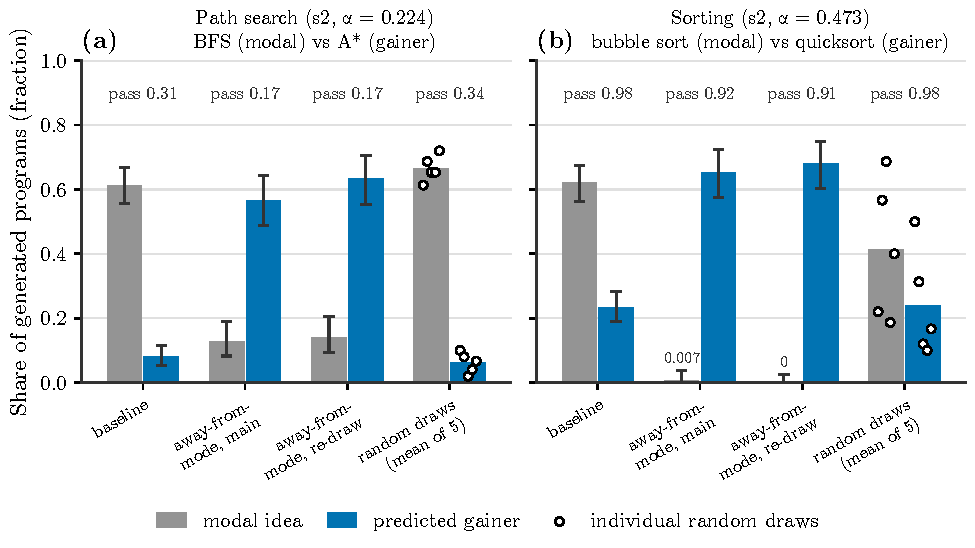
\includegraphics[width=0.80\linewidth,keepaspectratio]{figures/fig_selector_v0.pdf}
\caption{The headline test (gen\_art\_experiment\_6, round 2). Share of programs implementing the modal idea (grey) and the frozen predicted gainer (blue) at strength s2, for the baseline, the away-from-mode direction on the main draw and the fresh-seed re-draw, and the mean of five matched-norm random directions (open circles: individual draws). Error bars are Wilson 95\% intervals; the oracle pass rate is printed above each group.}
\end{figure}

\section*{5. What failed}

\begin{itemize}\setlength{\itemsep}{1pt}
\item \textbf{Flattening as a novelty knob} (round 1). Directions meant to flatten the idea utilities instead selected the minority idea. The held-out entropy ratio against temperature was 0.932 and 1.203, where 2 was required.
\item \textbf{Menu erasure and the cross-task ``unusualness dial''} (round 1). LEACE removed idea decodability, yet the outputs stayed BFS, DFS and Dijkstra. The dial was not monotone in strength (Spearman 0.486 and $-0.257$, exact p 0.356 and 0.658). No program the judge accepted as a novel correct algorithm appeared in any condition (0 of 70 checked).
\item \textbf{The pre-registered temperature law} (round 2). It was met on no task and draw: path-search intercepts reject pure temperature scaling, and the frozen law lost to fixed utilities on sorting out of sample.
\item \textbf{Seed strings as predictable shocks} (round 2). On sorting the predicted greedy flip rate was 0.394 and the observed rate 0.017; the internal readout failed its coverage gate.
\item \textbf{Internal geometry as the predictor of substitution} (round 2). The gain over IIA was 9.2\% where 20\% was required, top-substitute hits were 20\% where 70\% was required, and the predictor was worse than IIA on the k-th-smallest task and on gemma.
\item \textbf{The prompt-final state as the carrier of a ban} (round 2). Transplanting, subtracting or overwriting it moved nothing, on both models.
\item \textbf{Two round-1 claims withdrawn.} The claim that random directions raise entropy as much as targeted ones fails a draw-averaged comparison (3 targeted settings beat the draw mean, 5 fall below it, 10 are undetermined). The claim that ``bans are ignored'' holds only under the contract prompt with list wording.
\end{itemize}

\section*{6. Open questions}

\begin{itemize}\setlength{\itemsep}{1pt}
\item Where the idea is committed. Forking-path resampling was planned in both rounds and run in neither.
\item Whether the ban works as a prohibition or as name priming. Every regularity-violating ban names an in-domain algorithm, and the neutral-mention control was not run.
\item How the ban sentence is read during decoding. The knockout rests on four bans at n = 60. Knocking out the placebo sentence also shifts output, and no random-span control was run.
\item How specific the selector is. The off-target direction also raises A$^*$, and some random draws select on sorting.
\item Scope. One wording per condition and one Qwen size; gemma's path-search labels are label-limited (kappa 0.39); the user's two literal seed strings were never tested.
\end{itemize}

\small The full chronological record, with every table, is the 112-page internal report (\texttt{report.pdf}).

\end{document}
